% Settings for the default beamer theme
\documentclass[english, aspectratio=169]{beamer}
\usepackage[T1]{fontenc}
\usepackage[utf8]{inputenc}
\usepackage{tabularx}
\usepackage{babel}
\setcounter{secnumdepth}{3}
\setcounter{tocdepth}{3}

\makeatletter

\newcommand\makebeamertitle{\frame{\maketitle}}

% (ERT) argument for the TOC
\AtBeginDocument{%
  \let\origtableofcontents=\tableofcontents
  \def\tableofcontents{\@ifnextchar[{\origtableofcontents}{\gobbletableofcontents}}
  \def\gobbletableofcontents#1{\origtableofcontents}
}

% Theme settings
\usetheme{Frankfurt}
\usecolortheme{default}
\usefonttheme[onlymath]{serif}

% Template settings
\setbeamertemplate{navigation symbols}{}
\setbeamertemplate{blocks}[rounded][shadow=false]
\setbeamertemplate{title page}[default][colsep=-4bp, rounded=true, shadow=false]
\makeatother

\begin{document}

% Title page
\section{Bevezetés}
\title[]{Üzleti Intelligencia}
\subtitle{2. Előadás: Bevezetés a megerősítéses tanulásba}
\author[Kuknyó Dániel]{Kuknyó Dániel\\Budapesti Gazdasági Egyetem}
\date{2023/24\\1.félév}
\makebeamertitle

% Table of contents slide
\begin{frame}
\tableofcontents{}
\end{frame}

\begin{frame}
\tableofcontents[currentsection]
\end{frame}

\begin{frame}{A gépi tanulás fő területei}
A három fő típus, ahova be lehet sorolni a gépi tanulási algoritmusokat:
\begin{itemize}
	\item Felügyelt tanítás
	\item Felügyelet nélküli tanítás
	\item Megerősítéses tanulás
\end{itemize}
\begin{center}

\includegraphics[height=6cm, width=12cm, keepaspectratio]{images/reinf_21.png}
\end{center}
\end{frame}

\begin{frame}{Hol vagyunk?}
\begin{columns}
\begin{column}{.5\textwidth}
A megerősítéses tanulás számos tudományterület együttese.\par\smallskip
A fő elképzelése az, hogy az emberi illetve evolúcióból ismerős módszerekkel tanítson helyzethez alkalmazkodni tudó, intelligens modelleket valamilyen módszertan alapján. 
\end{column}
\begin{column}{.5\textwidth}
\begin{center}
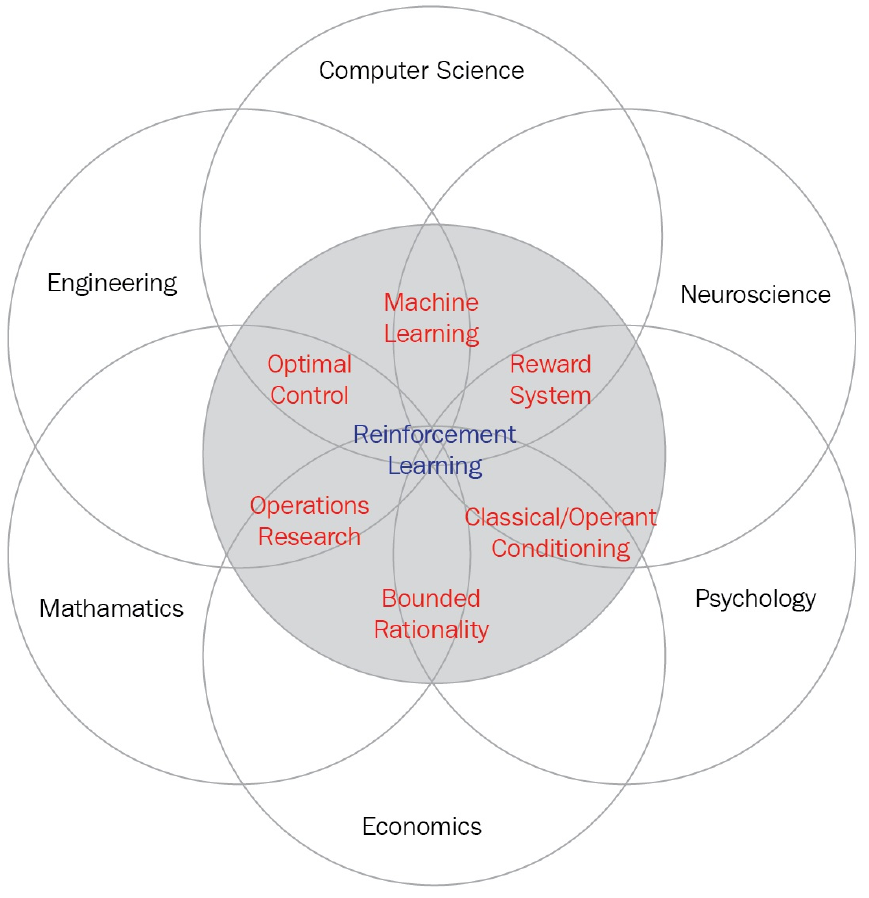
\includegraphics[height=7cm, width=12cm, keepaspectratio]{images/reinf_1.png}
\end{center}
\end{column}
\end{columns}
\end{frame}

\begin{frame}{A megerősítéses tanulás}
A megerősítéses tanuló modell célja, hogy \textbf{a legjobb döntéseket hozza egymás után}, egy adott kontextusban, hogy \textbf{maximalizálja a sikert mérő értéket}. A döntéshozó entitás próbákkal és hibákkal tanul. Nincs megadva, hogy milyen döntéseket hozzon, hanem ő maga tanulja meg azáltal, hogy kipróbálja azokat.
\begin{center}
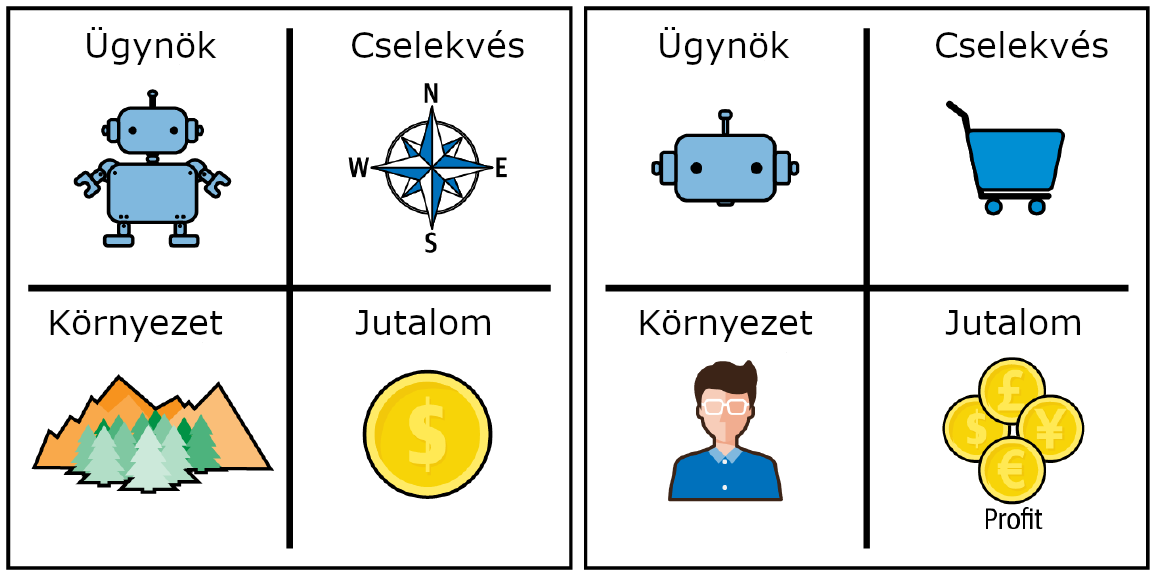
\includegraphics[width=12cm, height=5cm, keepaspectratio]{images/reinf_2.png}
\end{center}
\end{frame}

\begin{frame}{A modellezés komponensei}
\begin{columns}
\begin{column}{.3\textwidth}
\begin{center}
\only<1>{\begin{block}{Ügynök}
Az autonóm cselekvő, ami a feladat végrehajtására törekszik.
\end{block}}
\only<2>{\begin{block}{Környezet}
Egy fekete doboz, amely az ügynök cselekvéseinek helyszíne.
\end{block}}
\only<3>{\begin{block}{Idő}
RL folyamán az időlépések diszkrétek:\\
$t\in{1,2,3,...}$
\end{block}}
\only<4>{\begin{block}{Állapot}
Az ügynök megfigyelése a környezetre vonatkozóan. A környezetet leíró változók összessége.\\
Jelölés: $s\in{S}$, ahol $S$ az összes állapot halmaza.
\end{block}}
\only<5>{\begin{block}{Jutalom}
Az ügynök cselekvésének jóságát jelző skalár.\\
Jelölés: $r\in{\mathbb{R}}$
\end{block}}
\only<6>{\begin{block}{Cselekvés}
Az ügynök által végrehajtott művelet, ami a környezetet befolyásolja.\\
Jelölés: $a \in{A}$, ahol $A$ az összes cselekvés halmaza.
\end{block}}
\only<7>{\begin{block}{Politika}
Egy állapot $\rightarrow$ cselekvés leképezés. Az ügynök cselekvéseinek szabályait adja meg.\\
Jelölés:\\
\begin{itemize}
	\item Determinisztikus: $\pi\in{S\rightarrow}A$
	\item Sztochasztikus: $\pi\in{S\times}A\rightarrow [0,1]$\\
	Röviden: $\pi (s,a)$\\
	Vagy: $\pi (a|s)$
\end{itemize} 
\end{block}}
\end{center}
\end{column}
\begin{column}{.7\textwidth}
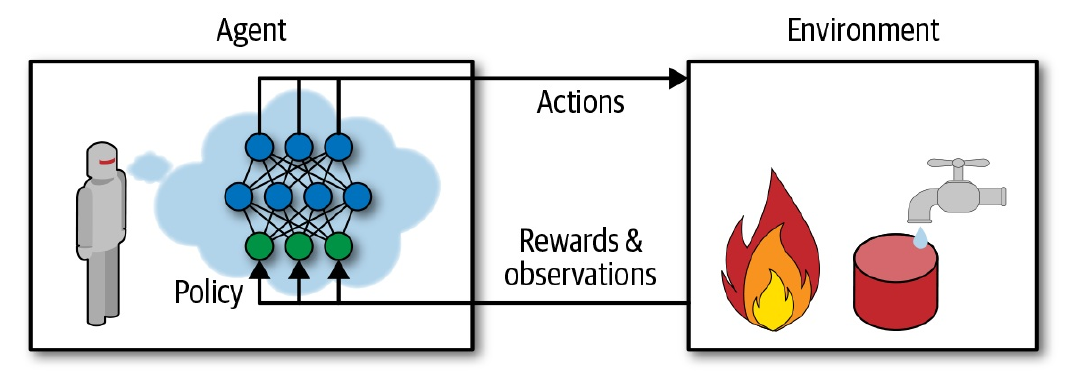
\includegraphics[width=10cm, keepaspectratio]{images/reinf_3.png}
\end{column}
\end{columns}
\end{frame}

\begin{frame}{Interakció a környezettel}
\begin{columns}
\begin{column}{.5\textwidth}
\begin{itemize}
	\item Az ügynök és a környezet egymásra hatnak. Az ügynök cselekszik, ennek hatására a környezet megváltozik. Az ügynök megfigyeli a környezetet, majd ismét cselekszik:
$s_1 \rightarrow a_1 \rightarrow s_2 \rightarrow a_2 \rightarrow ... \rightarrow s_t \rightarrow a_t$
	\item A jutalom azonnali, és cselekvés-állapot párosért jár: $R(s, a)$
	\item A környezet változását az átmeneti valószínűségek adják: $P(s'|s, a)$, ami $s'$ következő állapot valószínűsége $s$ állapotból, $a$ cselekvést követően. Ez a \textbf{környezet dinamikája}.
\end{itemize}
\end{column}
\begin{column}{.5\textwidth}
\begin{itemize}
	\item Az ügynök célja a lehető legmagasabb jutalom összegyűjtése hosszú távon: 
	\[
	E_{\pi}(r_{1}+r_{2}+r_{3}+...)\rightarrow{max}
	\]
\end{itemize}
\begin{center}
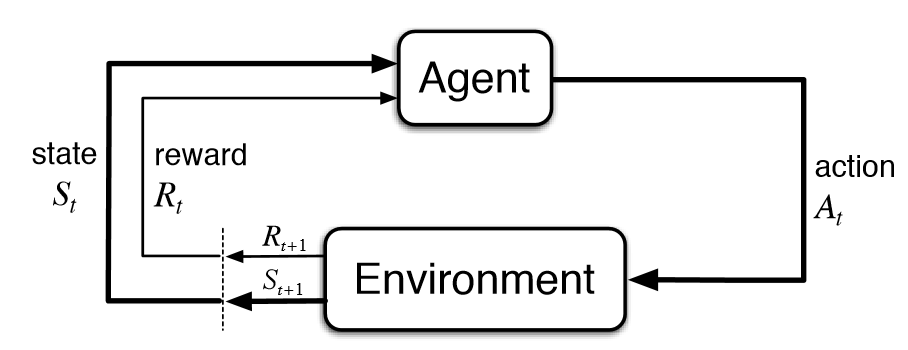
\includegraphics[width=7.5cm, keepaspectratio]{images/reinf_4.png}
\end{center}
\end{column}
\end{columns}
\end{frame}

\begin{frame}{A kredit hozzárendelési probléma}
\begin{columns}
\begin{column}{.5\textwidth}
\only<1>{A megerősítéses tanulásban a jutalmak általában ritkák és késleltetettek.\\
Például: ha az ügynök életben maradt 100 lépésen keresztül, és a 101. lépésben meghal, honnan tudjuk, melyik lépés volt érte a felelős?\par\smallskip
A probléma megoldására a tanulás egy diszkont rátát ($\gamma$) alkalmaz.\\
A diszkont ráta megadja a jövőbeli jutalmak jelenbeli értékét. Valamely $r$ jutalom értéke $k$ időlépés után $\gamma^{k-1}$.} 
\only<2>{Ha az ügynök  háromszor egymás után jobbra megy, és $+10$ jutalmat kap az első lépés után, $0$-t a második lépés után, és végül $-50$-et a harmadik lépés után, akkor feltéve, hogy $\gamma=0.8$ diszkontálási tényezőt használ, az első lépés hozama $10+\gamma 0+\gamma^2 (-50)=-22$ lesz. \par\smallskip
Ha a diszkontálási tényező közel van a $0$-hoz, akkor a jövőbeli jutalmak nem számítanak sokat az azonnali jutalmakhoz képest. Ha viszont a diszkontálási tényező közel van $1$-hez, akkor a jutalmak a jövőben majdnem ugyanannyit számítanak, mint az azonnali jutalmak.}
\end{column}
\begin{column}{.5\textwidth}
\begin{center}
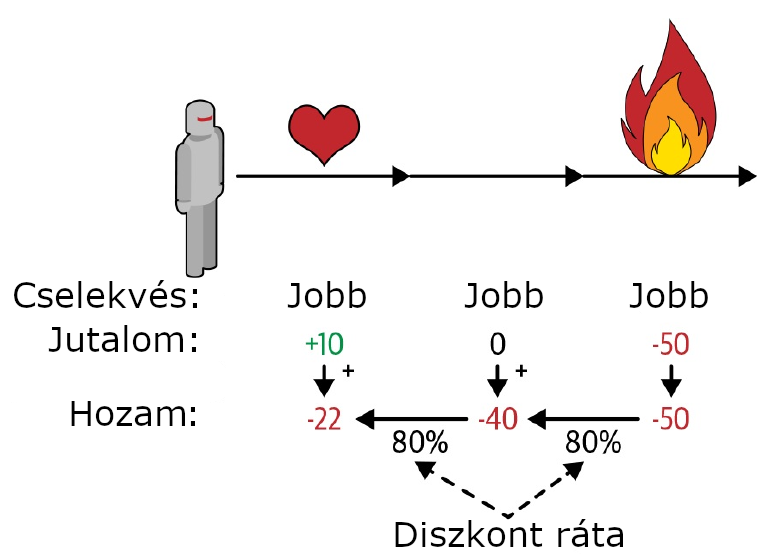
\includegraphics[width=7cm, keepaspectratio]{images/reinf_5.png}
\end{center}
\end{column}
\end{columns}
\end{frame}

\section{Markov döntési folyamatok}

\begin{frame}
\tableofcontents[currentsection]
\end{frame}

\begin{frame}{Markov láncok}
\begin{center}
\begin{columns}
\begin{column}{.5\textwidth}
\only<1>{\begin{block}{Markov lánc}
\textbf{Memória nélküli sztochasztikus folyamat} fix számosságú állapottal, amely véletlenszerűen vált állapotot minden lépésben.\\
Az átmeneti valószínűség az aktuális állapotból ($s$) a következő állapotba ($s'$) előre meghatározott, és csak az $(s, s')$ pároson múlik, múltbeli állapotokon nem. 
\end{block}}
\only<2>{\begin{block}{Markov tulajdonság}
Az ügynök nem nyerhet semmit azáltal, hogy ismeri az előző állapotokat.
\end{block}
\begin{itemize}
	\item Miért fontos ez?
	\item Milyen példákat lehet mondani ilyen játékokra?
\end{itemize}}
\end{column}
\begin{column}{.5\textwidth}
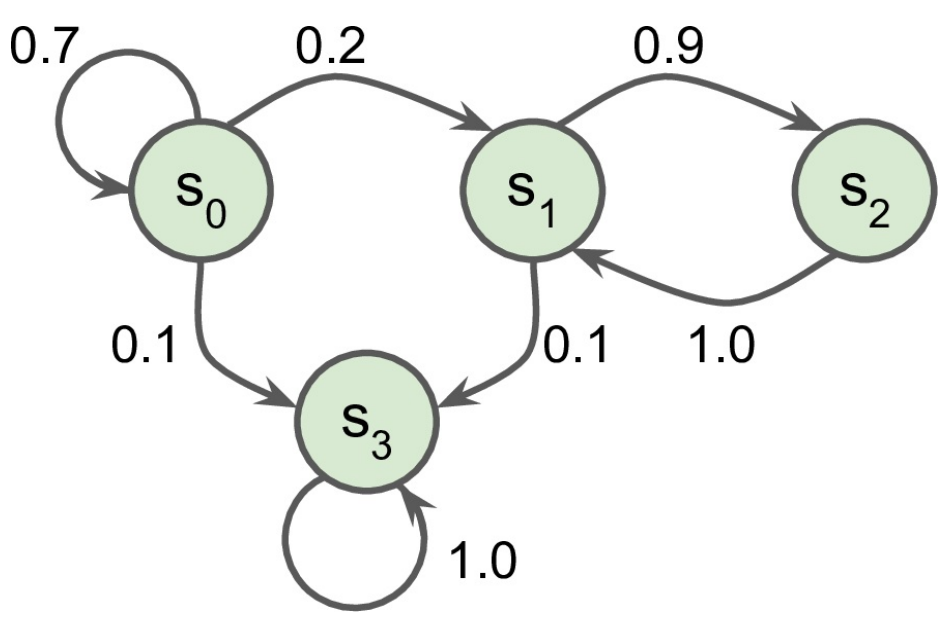
\includegraphics[width=7cm, height=12cm, keepaspectratio]{images/reinf_6.png}
\end{column}
\end{columns}
\end{center}
\end{frame}

\begin{frame}{Markov döntési folyamatok}
\begin{columns}
\begin{column}{.5\textwidth}
\only<1>{\begin{block}{Markov döntési folyamat (MDP)}
Az ügynök minden lépésben választhat egy cselekvés közül. A környezet állapot átmeneti valószínűsége a következő állapotba a választott cselekvésen fog múlni. Ezenkívül némelyik állapot átmenetek jutalommal (pozitív vagy negatív) járnak.
\end{block}}
\only<2>{Ha az ügynök az $s_0$ állapotban kezd, választhat az $a_0$, $a_1$ vagy $a_2$ cselekvések között. Ha az $a_1$ cselekvést választja, biztosan az $s_0$ állapotban marad jutalom nélkül. De ha az $a_0$ cselekvést választja, akkor $70\%$ esélye van arra, hogy $+10$ jutalmat kapjon és az $s_0$ állapotban maradjon. Előbb-utóbb az $s_1$ állapotba fog megérkezni. Itt csak két lehetséges cselekvés van: $a_0$ és $a_2$. Az $a_0$ cselekvéssel ugyanabban az állapotban marad, vagy továbblép az $s_2$ állapotba és $-50$ jutalmat kap. Az $s_2$ állapotban csak az $a_1$ cselekvést teheti meg, amely visszavezeti az $s_0$ állapotba, $+40$ jutalommal.}
\end{column}
\begin{column}{.5\textwidth}
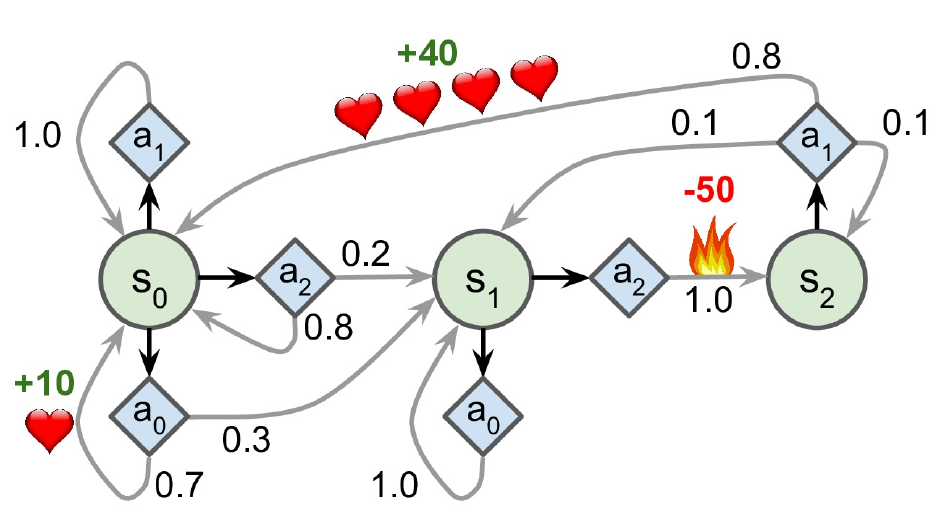
\includegraphics[width=7cm, height=12cm, keepaspectratio]{images/reinf_7.png}
\end{column}
\end{columns}
\end{frame}

\begin{frame}{A Markov döntési folyamat medoldása}
\begin{columns}
\begin{column}{.6\textwidth}
A probléma felírása: 
\begin{itemize}
	\item Az ügynök $s_0$ kezdőállapotból indul.
	\item Minden cselekvését $\pi$ politika határozza meg.
	\item A környezet az állapot és a cselekvés alapján ad jutalmat:\\
	$s_{t+1}\sim{P(s_{t}, a_{t})};\;r_{t+1}\sim{R(s_{t}, a_{t})}$
	\item A politika optimális, ha a kumulált diszkontált jutalma (\textbf{hozama}) maximális:\\
	\begin{block}{}
	\[	
	G_{t} = (r_{1} + \gamma r_{2} + \gamma ^2 r_{3} + ...)=
	\]
	\[	
	=\sum_{k=0}^{\infty}\gamma^{k}r_{t+k+1} \rightarrow max
	\]
	\end{block}
\end{itemize}
\end{column}
\begin{column}{.4\textwidth}
\begin{itemize}
	\item A cél az \textbf{optimális politika} megtalálása.
\end{itemize}
\begin{center}
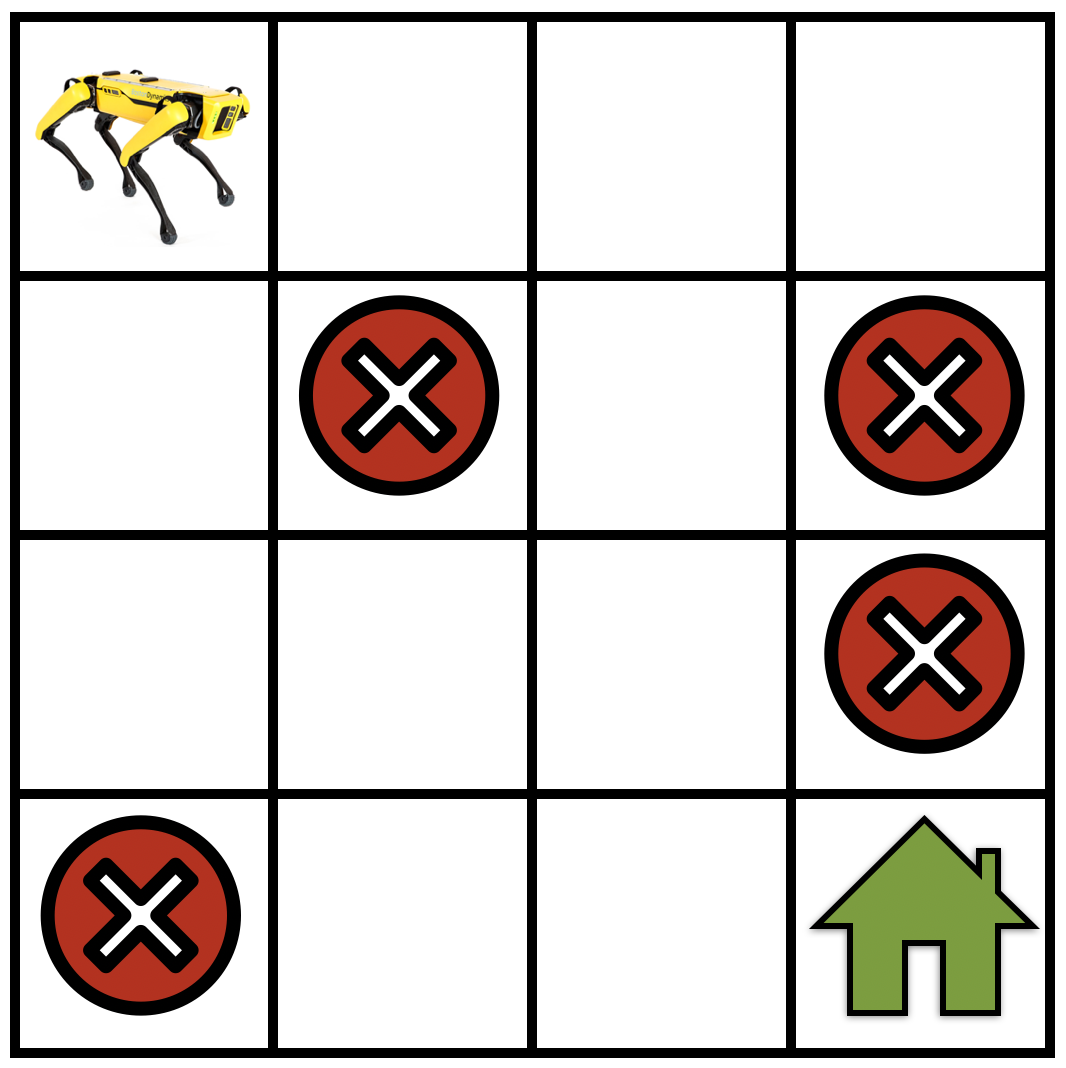
\includegraphics[width=4cm, height=5cm, keepaspectratio]{images/reinf_8.png}
\end{center}
\end{column}
\end{columns}
\end{frame}

\section{Értékfügvények}

\begin{frame}
\tableofcontents[currentsection]
\end{frame}

\begin{frame}{Állapot-érték függvény}
\begin{columns}
\begin{column}{.5\textwidth}
Az értékfüggvények az állapotok függvényei amik megadják, hogy mennyire jó az ügynöknek, hogy egy adott állapotban áll.
\begin{block}{Állapot-érték függvény (value)}
Egy $s$ állapot állapot-értéke ($v_{\pi}(s)$) valamely $\pi$ politika szerint a várható hozam, ha az ügynök $s$ állapotból indul, és utána $\pi$ szerint hozza döntéseit:\\
\[
V_{\pi}(s)=E_{\pi}\left[G_{t}|S_{t}=s\right]=
\]
\[
=E_{\pi}\left[\sum_{k=0}^{\infty}\gamma^{k}r_{t+k+1}\mid S_{t}=s\right]
\]
\end{block}
\end{column}
\begin{column}{.5\textwidth}
\begin{center}
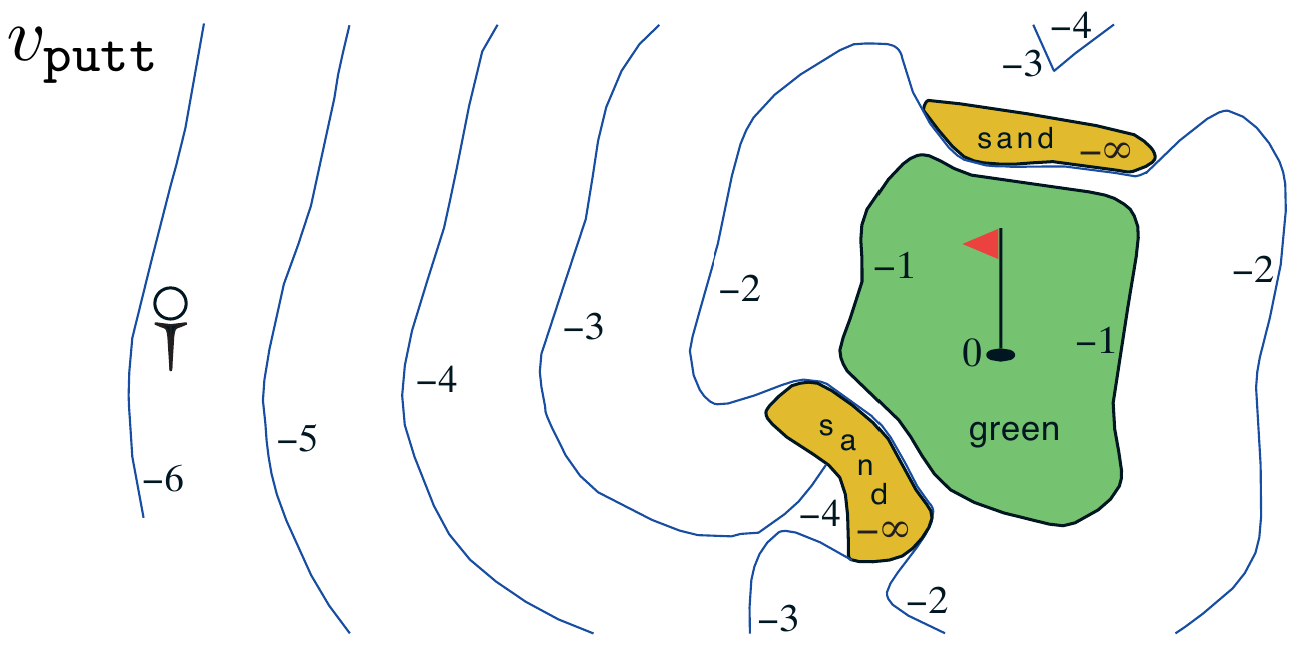
\includegraphics[width=5cm, height=5cm, keepaspectratio]{images/reinf_9.png}
\end{center}
\begin{small}
Példa: golfozásban a \emph{putter} a kis hatótávú golfütőre vonatkozik. A diagramon azt látjuk, mennyire jó egy adott pozícióból ütni annak az ügynöknek, aki csak a putter ütőt használja. A terminális állapotban az érték $0$, és minél távolabb van tőle, annál inkább csökken az értéke. A homokon a politika $-\infty$ értéket kap.
\end{small}
\end{column}
\end{columns}
\end{frame}

\begin{frame}{Állapot-értékek a Breakout-ban}
A Breakout egy retró Atari játék, amiben a cél az, hogy az ütővel a játékos leüsse az összes téglát. A diagramon az adott állapothoz tartozó állapot-érték látható. Amikor felkerül a labda az állapot-érték is magasabb, mert ott potenciálisan több téglát tud kiütni. 
\begin{center}
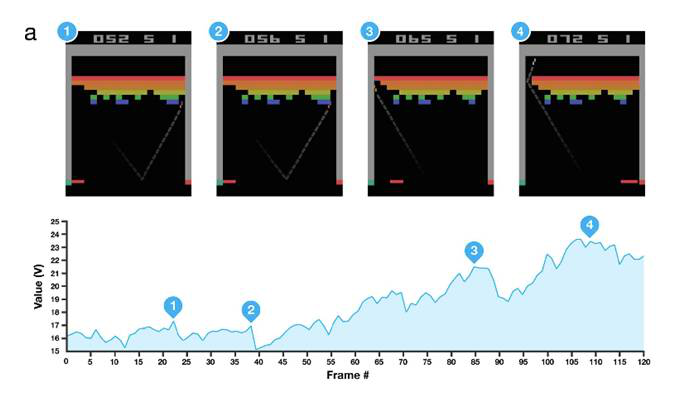
\includegraphics[width=9cm, height=7cm, keepaspectratio]{images/breakout.png}
\end{center}
\end{frame}

\begin{frame}{Állapot-cselekvés minőség függvény}
\begin{columns}
\begin{column}{.62\textwidth}
Hasonlóan az előzőhöz lehetséges definiálni egy adott állapot-cselekvés páros minőségének függvényét, amely megadja mennyire jó az ügynöknek, hogy egy adott állapotban áll, majd adott cselekvést hajt végre.
\begin{block}{Állapot-cselekvés minőség függvény (quality)}
Egy $(s,a)$ állapot-cselekvés páros minőség függvénye valamely $\pi$ politika szerint a várható hozam, ha az ügynök $s$ állapotból indul, $a$ cselekvést hajtja végre, majd utána $\pi$ szerint hozza döntéseit:\\
\[
Q_{\pi}(s,a)=E_{\pi}\left[G_{t}|S_{t}=s,A_{t}=a\right]=
\]
\[
=E_{\pi}\left[\sum_{k=0}^{\infty}\gamma^{k}r_{t+k+1}\mid S_{t}=s,A_{t}=a\right]
\]
\end{block}
\end{column}
\begin{column}{.4\textwidth}
\begin{center}
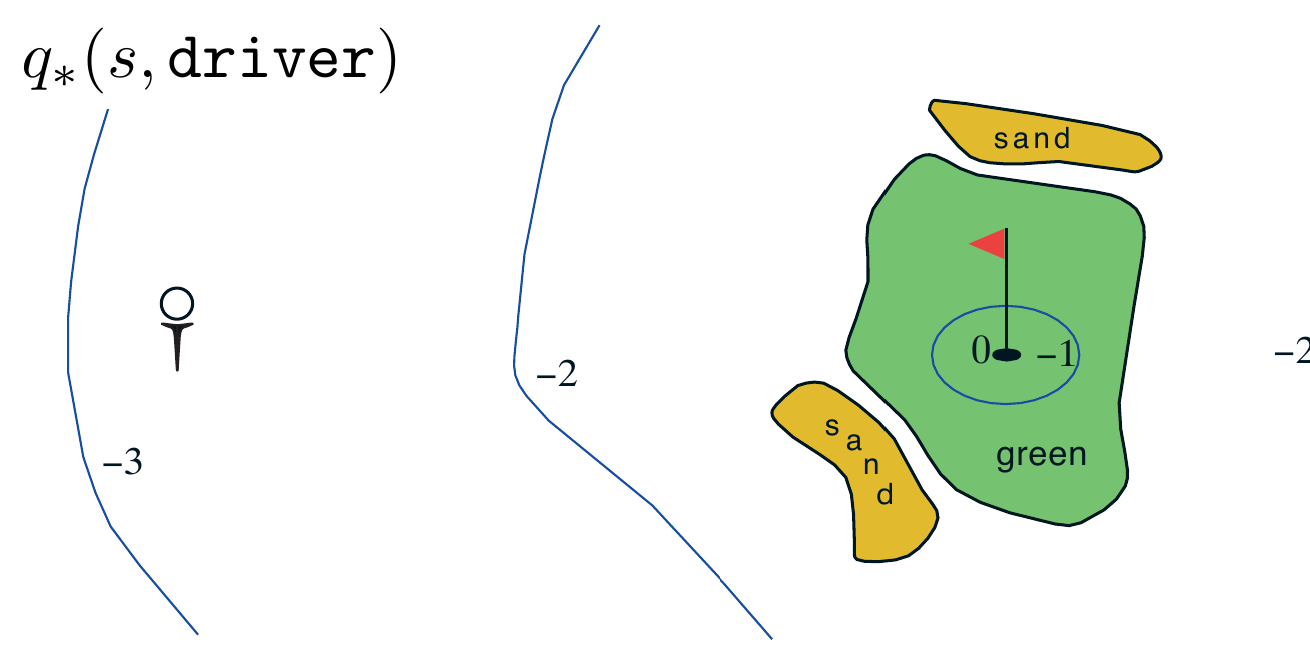
\includegraphics[width=5cm, height=5cm, keepaspectratio]{images/reinf_10.png}
\end{center}
\begin{small}
Példa: golfozásban a \emph{driver} a nagy  hatótávú ütőre vonatkozik. Ebben az esetben a $q(s, driver)$ minőség függvény azt adja meg mennyire jövedelmező a játékosnak egy adott helyen állni, és onnan a driver ütőt választani a következő lövéshez.
\end{small}
\end{column}
\end{columns}
\end{frame}

\section{Bellman szabályok}

\begin{frame}
\tableofcontents[currentsection]
\end{frame}

\begin{frame}{Állapot-érték Bellman szabály}
\begin{columns}
\begin{column}{.6\textwidth}
Az értékfüggvények egy alapvető tulajdonsága, hogy betartanak egy rekurzív kapcsolati rendszert. Minden $\pi$ politikára és bármely $s$ állapot esetén érvényes a következő konzisztencia kritérium $s$ állapot és $s'$ következő állapotai között:
\begin{block}{Állapot-érték Bellman szabály}
\[
V_{\pi}(s)=\sum_{a}\pi(a|s)\sum_{s',r}p\left(s',r|s,a\right)\left[r+\gamma v_{\pi}\left(s'\right)\right]
\]\\
$\;minden\;s\in S-re$
\end{block}
\end{column}
\begin{column}{.45\textwidth}
\begin{center}
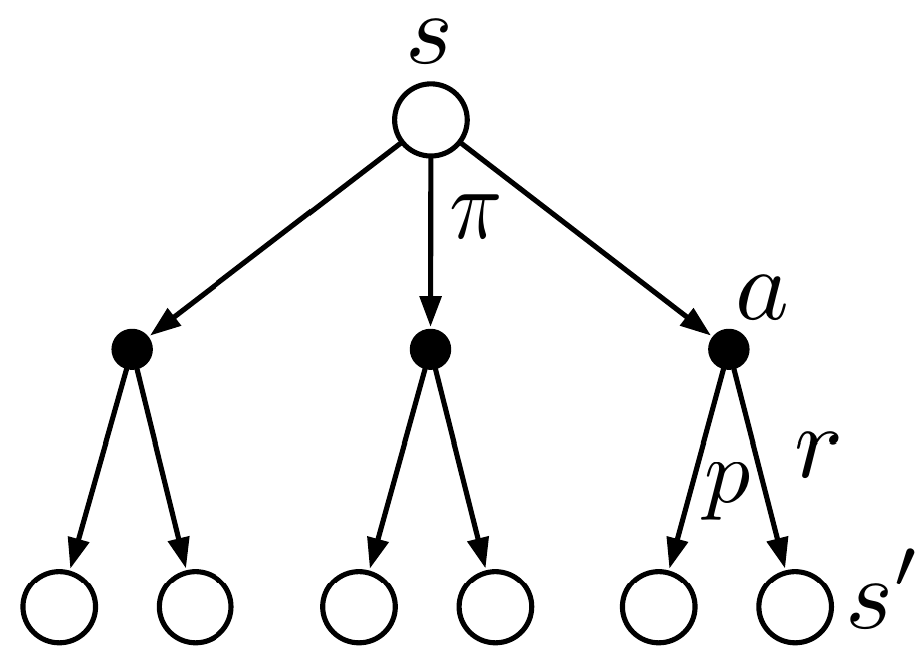
\includegraphics[width=5cm, height=5cm, keepaspectratio]{images/reinf_11.png}
\end{center}
\begin{itemize}
	\item $\pi(a|s)$: $a$ cselekvés valószínűsége $s$ állapotból $\pi$ politika szerint.
	\item $p\left(s',r|s,a\right)$: $s'$ következő állapot és $r$ jutalom valószínűsége, ha adott $s$ állapot és $a$ cselekvés.
\end{itemize}
\end{column}
\end{columns}
\end{frame}

\begin{frame}{Állapot-cselekvés minőség Bellman szabály}
\begin{columns}
\begin{column}{.6\textwidth}
Hogyan lehet javítani egy $\pi$ politikát?\\
Azt tudjuk, hogy mennyire jövedelmező egy $s$ állapotból $\pi$-t követni - ez a $v_\pi(s)$.\\ Érdemes lenne eltérni $\pi$ politikától egy adott $a$ cselekvést választva?\par\smallskip
Ezt adja meg az állapot-cselekvés minőség függvény: mennyire jövedelmező egy ügynöknek $s$ állapotból $a$ cselekvést választani, majd utána $\pi$ politikát követni:\\
\begin{block}{Állapot-cselekvés minőség Bellman szabály}
\[
Q_{\pi}(s,a)=\sum_{s',r}p\left(s',r|s,a\right)\left[r+\gamma v_{\pi}\left(s'\right)\right]
\]
\end{block}
\end{column}
\begin{column}{.45\textwidth}
\begin{center}
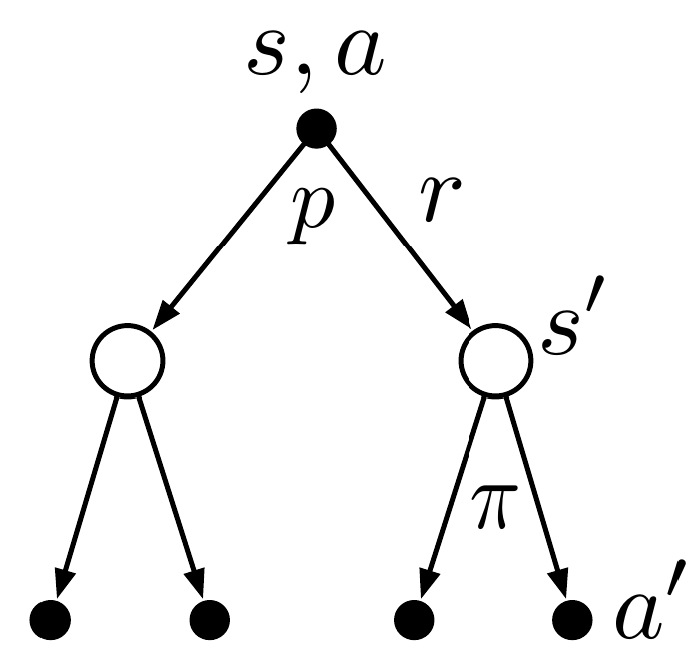
\includegraphics[width=5cm, height=5cm, keepaspectratio]{images/reinf_12.png}
\end{center}
\begin{itemize}
	\item $p\left(s',r|s,a\right)$: $s'$ következő állapot és $r$ jutalom valószínűsége, ha adott $s$ állapot és $a$ cselekvés.
\end{itemize}
\end{column}
\end{columns}
\end{frame}

\section{Politika javítása}

\begin{frame}
\tableofcontents[currentsection]
\end{frame}

\begin{frame}{Mohó ügynök}
\begin{columns}
\begin{column}{.5\textwidth}
Hogyan válasszon cselekvést az ügynök?\\
A legegyszerűbb cselekvés kiválasztási szabály, ha az ügynök mindig a számára elérhető legnagyobb értékű cselekvést választja. Ha több ilyen is van, tetszőlegesen választhat közöttük. 
\begin{center}
\begin{block}{Mohó cselekvés választás}
\[
a_{t}=\underset{a}{argmax}\:Q_{t}(a)
\]
\end{block}
\begin{itemize}
	\item Mindig a mohó a legjobb megoldás?
	\item A legjobb megoldás mohó?
\end{itemize}
\end{center}
\end{column}
\begin{column}{.5\textwidth}
\begin{center}
\only<1>{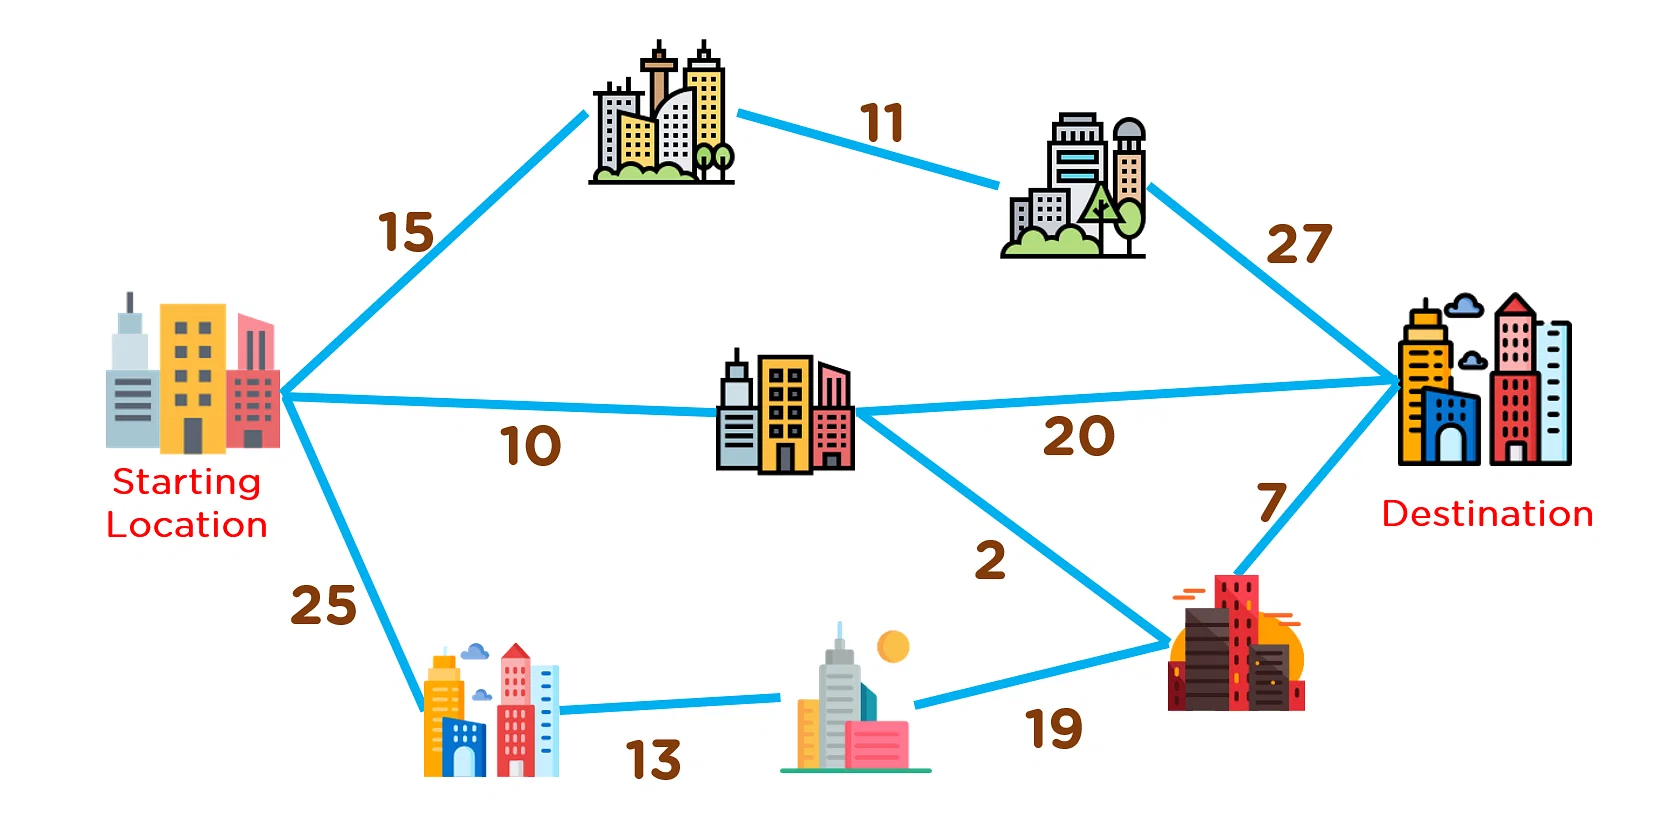
\includegraphics[width=7cm, height=7cm, keepaspectratio]{images/reinf_13.png}}
\only<2>{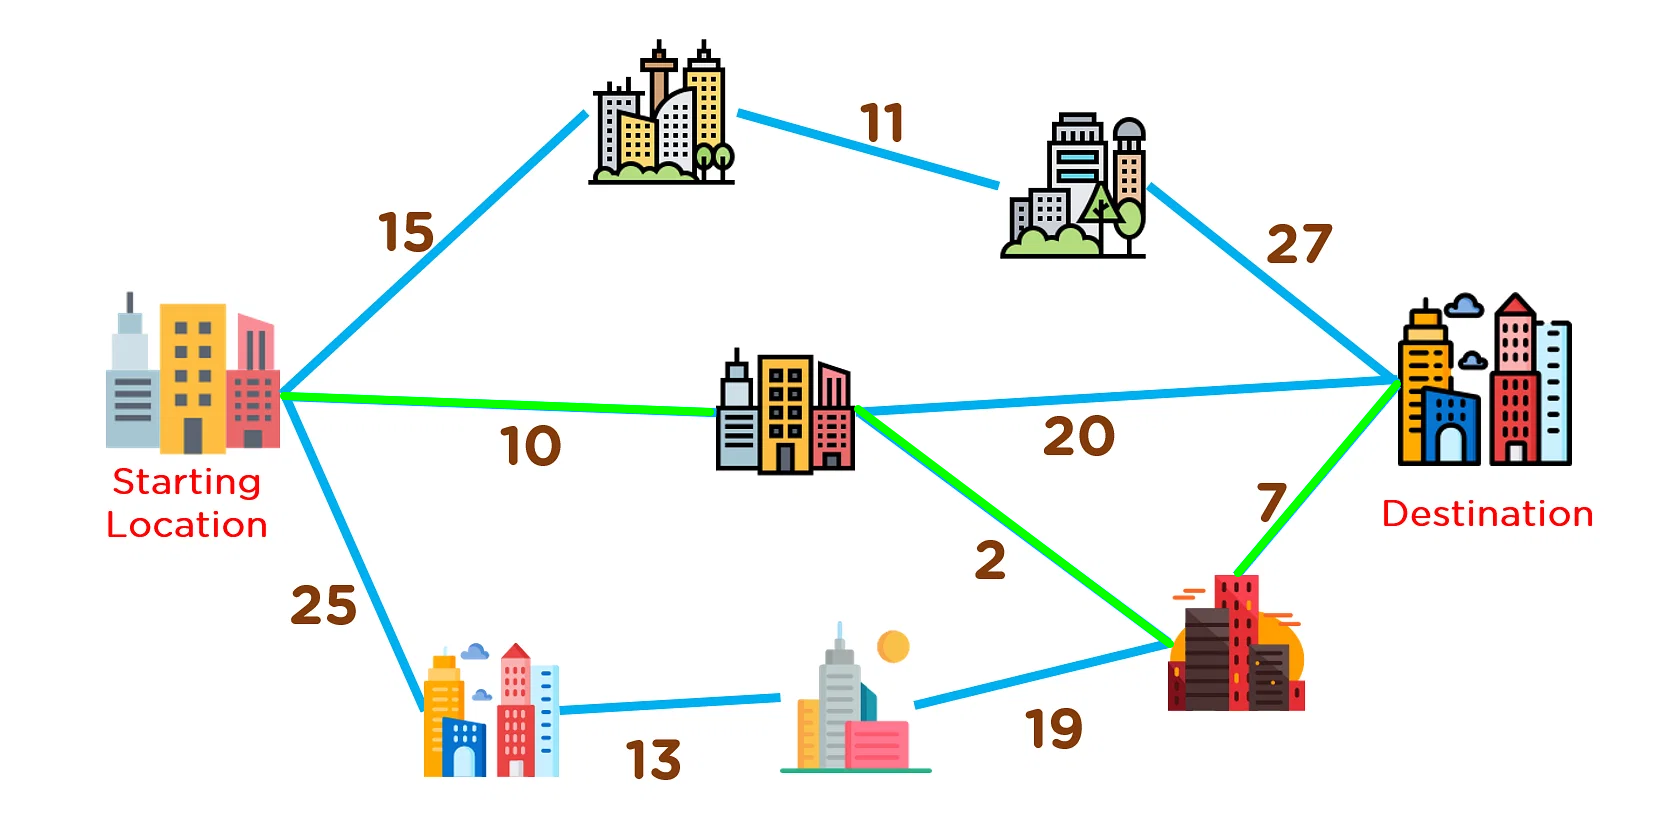
\includegraphics[width=7cm, height=7cm, keepaspectratio]{images/reinf_14.png}}
\end{center}
Melyik úton jutna el a mohó ügynök a kezdő városból a cél városba, ha a lehető legkevesebbet akarja költeni üzemanyagra?
\end{column}
\end{columns}
\end{frame}

\begin{frame}{GridWorld}
A példában egy egyszerű GridWorld játéknak láthatóak az állapot-értékei (jobb) és a mohó ügynök adott állapot-értékhez tartozó cselekvései politika javítás során. A játék célja, hogy az ügynök elérje valamelyik szürke zónát.
\begin{center}
Véletlen politika értéke $(V_{k})\;\;\;\;\;\;\;\;\;\;\;\;\;\;\;$Mohó stratégia $V_{k}$ szerint
\only<1>{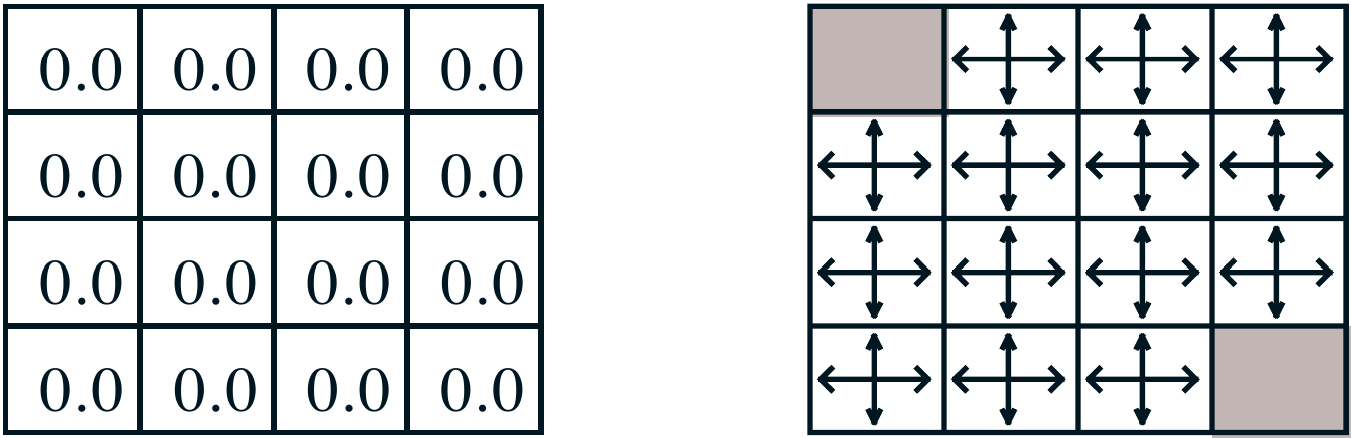
\includegraphics[width=10cm, height=7cm, keepaspectratio]{images/reinf_15.png}\\$k=0$}
\only<2>{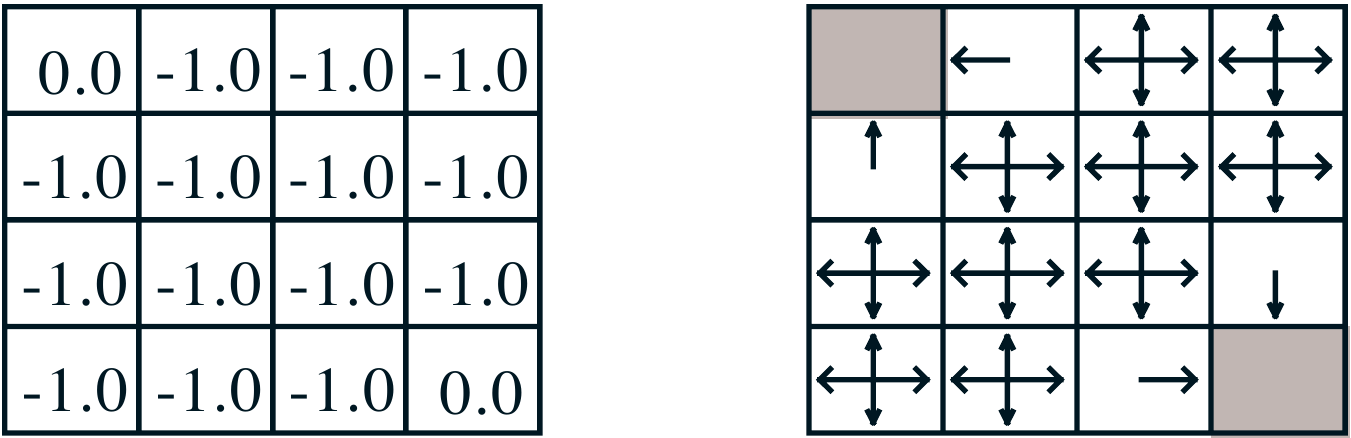
\includegraphics[width=10cm, height=7cm, keepaspectratio]{images/reinf_16.png}\\$k=1$}
\only<3>{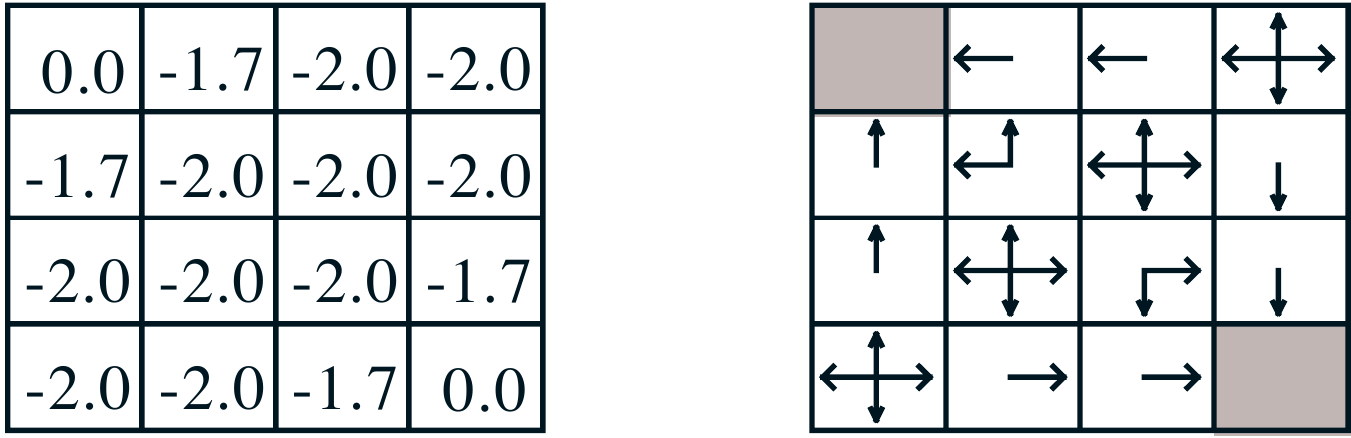
\includegraphics[width=10cm, height=7cm, keepaspectratio]{images/reinf_17.png}\\$k=2$}
\only<4>{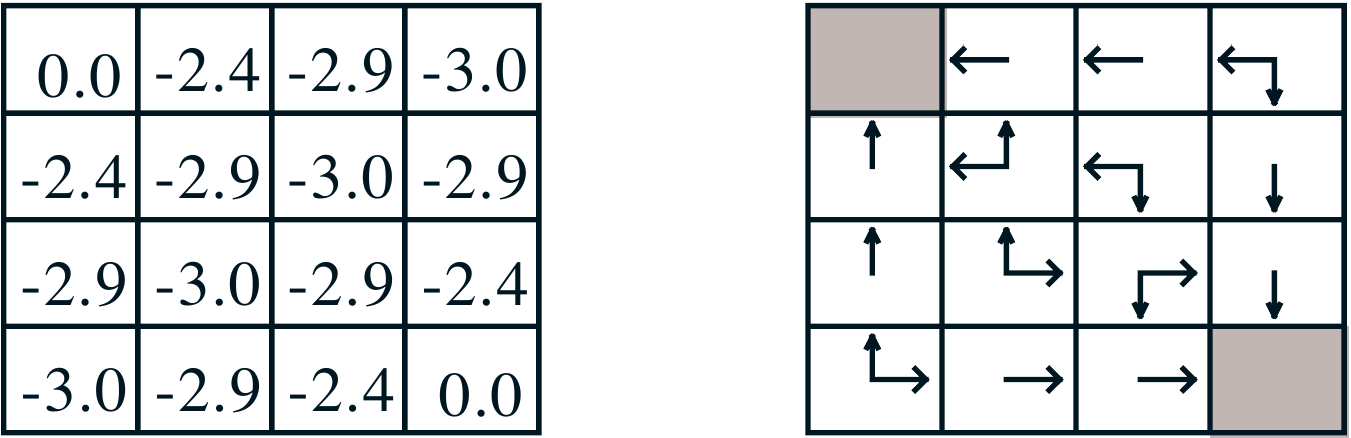
\includegraphics[width=10cm, height=7cm, keepaspectratio]{images/reinf_18.png}\\$k=3$}
\only<5>{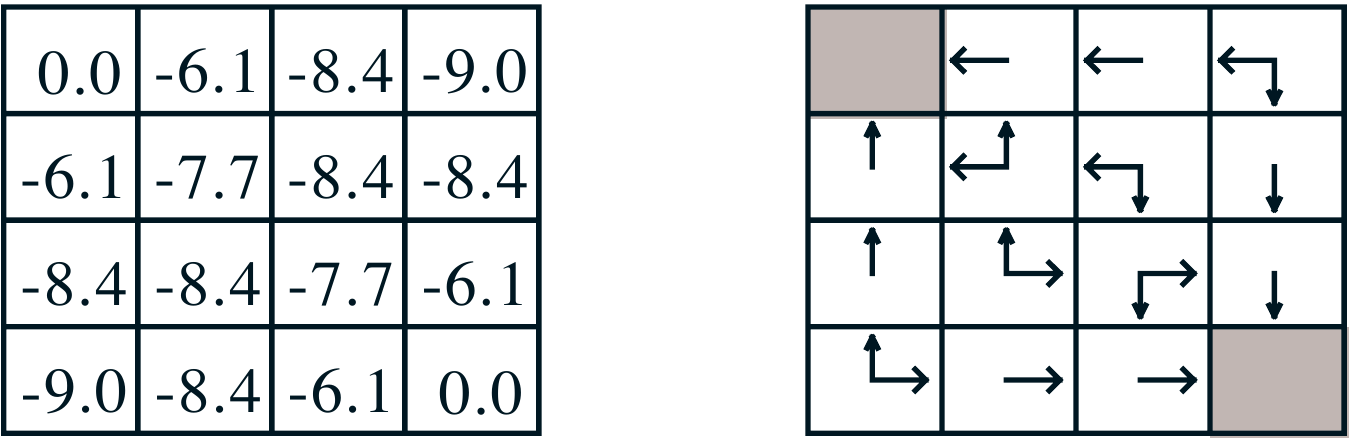
\includegraphics[width=10cm, height=7cm, keepaspectratio]{images/reinf_19.png}\\$k=10$}
\only<6>{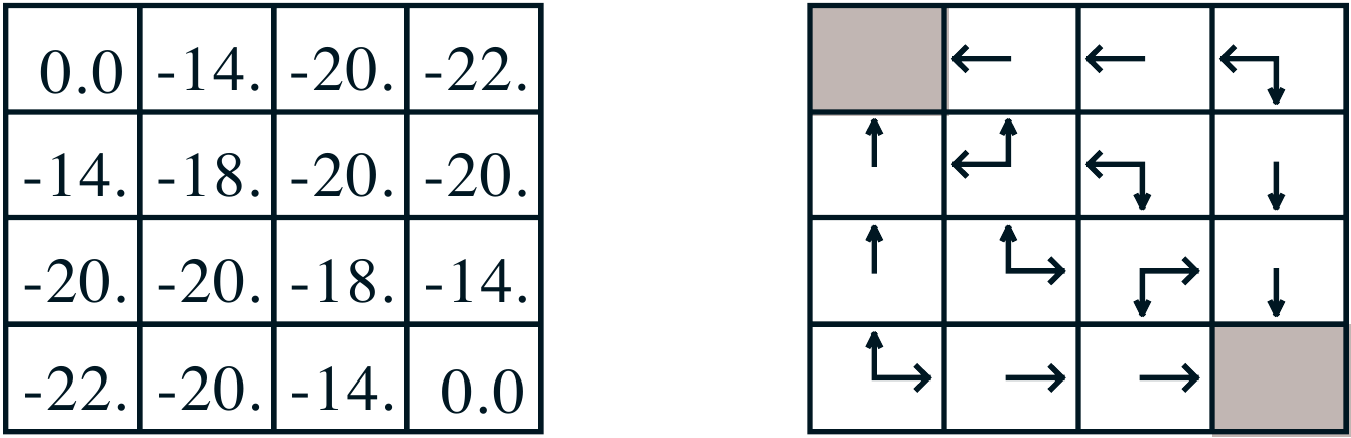
\includegraphics[width=10cm, height=7cm, keepaspectratio]{images/reinf_20.png}\\$k=\infty$}
\end{center}
\end{frame}

\end{document}














